\documentclass[11pt, a4paper]{jsarticle}
\usepackage{multicol}  % パッケージの追加
\usepackage[dvipdfmx]{graphicx}
\begin{document}
%=============================================================
%=============================================================
\section{Diffraction from circular apertures and slits}
\subsection*{Purpose}
実験の目的は円形開口やスリットの干渉模様の観察し,干渉から開口の直径,スリット幅,ダブルスリットの間隔を計算することである.
\subsection{Circular aperture}
\subsubsection{Procedure}
図\ref{fig:five}に示すように光学系を組み立てる.
またそれぞれの距離を図\ref{fig:five}に示すように名前をつける.
まず,レーザーの前に円形開口を置きそこから離れた距離にスクリーンを設置する.
今回は$02mm$,$0.4mm$の二つの円形開口を用いて実験を行う.
また,スクリーンは方眼紙で製作する.
次に開口からクリーンまでの距離$L$を測定する.
レーザーの電源をつけるとスクリーンに円形の干渉縞を得る.
次に円形の干渉縞の中心から1番目の暗線のまでの距離$r$を測定する.
これを二種類の円形開口に対して距離$L$を変えながら二回ずつ計測を行う.
\begin{figure}[htbp]
 \begin{center}
  \includegraphics[width=100mm]{fig5.png}
 \end{center}
 \caption{円形開口の光学系}
 \label{fig:five}
\end{figure}\\

またこれらの測定した距離は式(\ref{eq:b})の関係をみたす.
\begin{equation}
    sin\theta = \frac{1.22\lambda}{D} \label{eq:b}
\end{equation}\\


またこの時$\theta$,$D$の値は非常に小さいので$sin\theta \simeq tan\theta = r/L$とみなすことができる.
また今回使用したHe-Ne Laserの波長は$\lambda = 632.8nm$である.
以上より計測値を関係式へ代入して円形開口の直径を推測する.
その後0.2mm円形開口を光学顕微鏡によって計測しその直径を実際に求めた.

\subsubsection{Result}
測定結果から次の表が得られた.
\begin{table}[htb]
 \begin{minipage}{0.45\hsize}
  \begin{center}
    \caption{$0.2mm$円形開口}
    \begin{tabular}{rrr} \hline
        $r(mm)$ & $L(mm)$ & $D(mm)$  \\ \hline
        0.25     & 583 & 0.18\\
        0.45    & 1435 & 0.246\\ \hline
    \end{tabular}
    \label{tab:b}
  \end{center}
 \end{minipage}
 \begin{minipage}{0.45\hsize}
  \begin{center}
    \caption{$0.4mm$円形開口}
    \begin{tabular}{rrr} \hline
        $r(mm)$ & $L(mm)$ & $D(mm)$  \\ \hline
        2.6   & 974 & 0.289\\
        3.5    & 1430 & 0.315\\ \hline
    \end{tabular}
    \label{tab:c}
  \end{center}
 \end{minipage}
\end{table} 


またそれぞれ以下のような干渉模様が観測できた.
\begin{figure}[htbp]
 \begin{minipage}{0.45\hsize}
  \begin{center}
   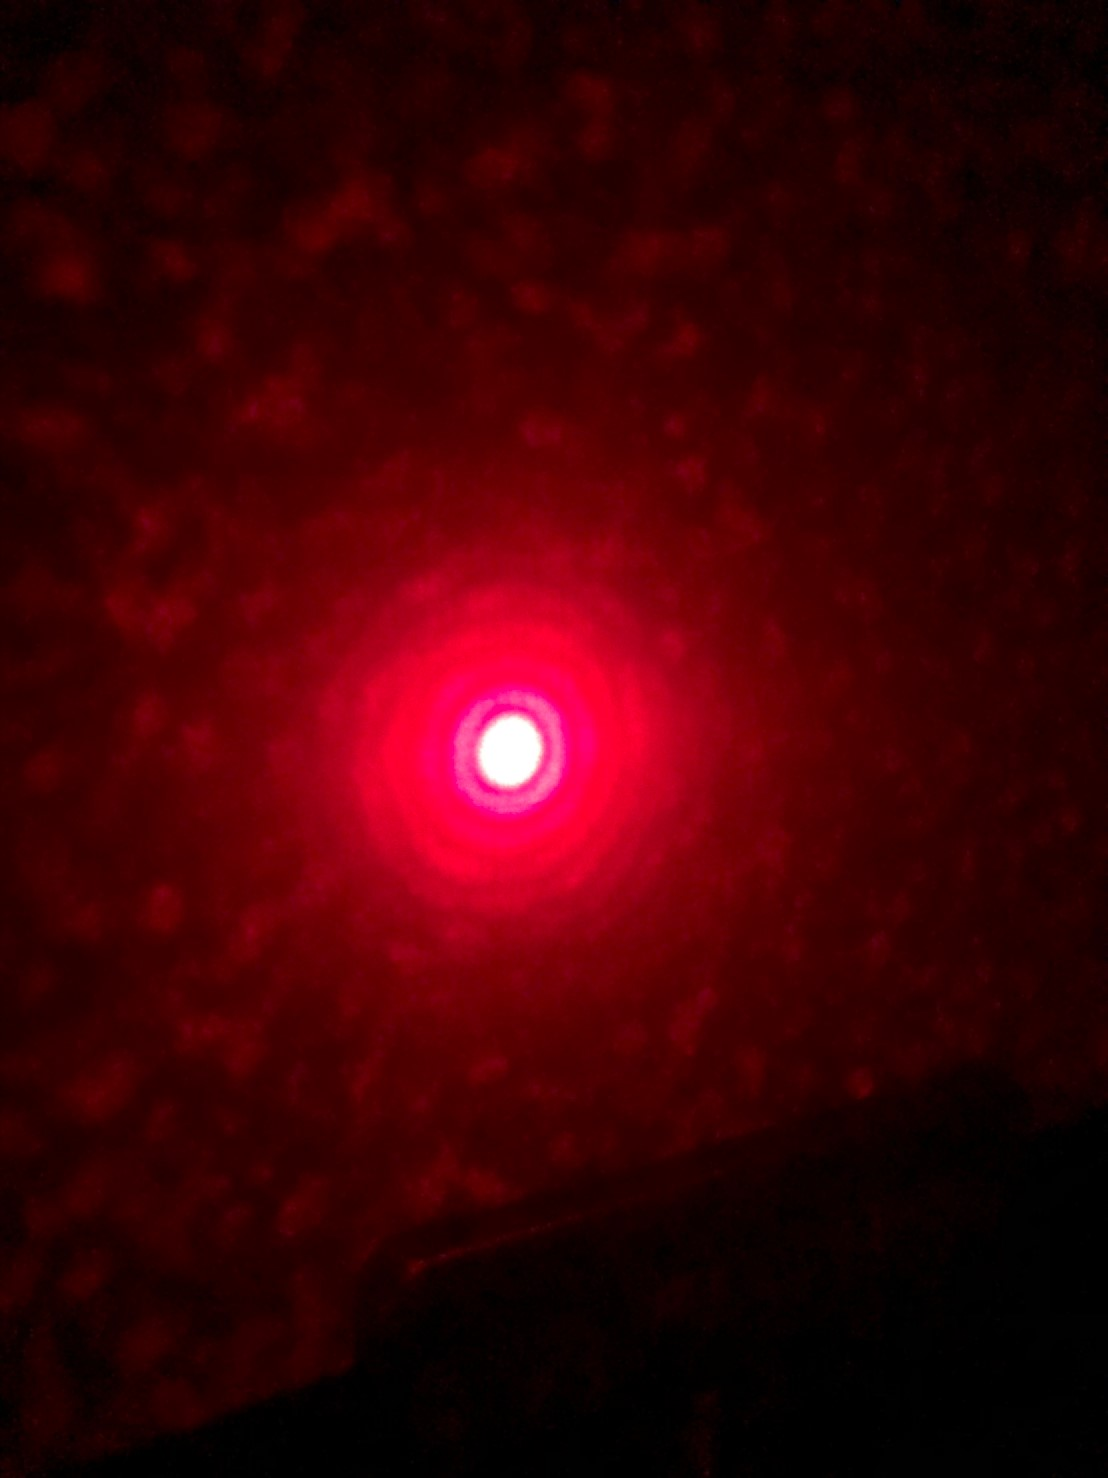
\includegraphics[width=60mm]{fig6.png}
  \end{center}
  \caption{$0.2mm$円形開口の干渉縞}
  \label{fig:six}
 \end{minipage}
 \begin{minipage}{0.45\hsize}
  \begin{center}
   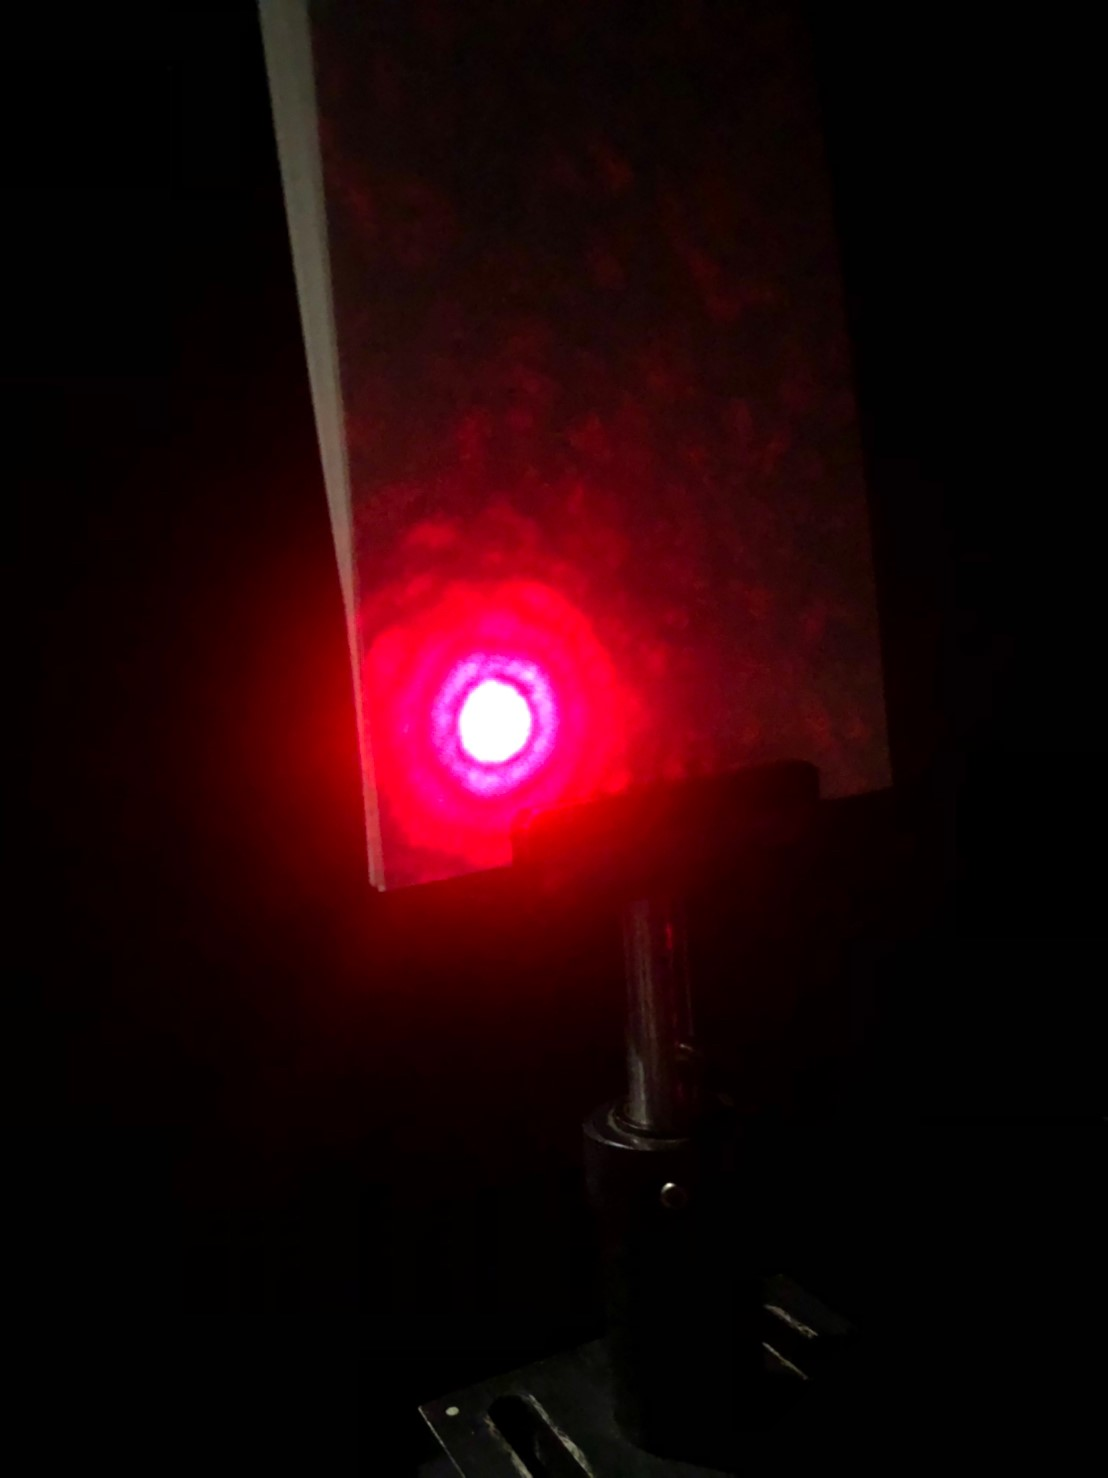
\includegraphics[width=60mm]{fig7.png}
  \end{center}
  \caption{$0.4mm$円形開口の干渉縞}
  \label{fig:seven}
 \end{minipage}
\end{figure}

また0.2mm円形開口の実測値は0.19mmであった.
干渉模様は円の半径が大きくなっていくに連れて明暗の境目が不明瞭になって区別がつかなくなった.

\newpage
また以下は光学顕微鏡で観測した0.2mm円形開口の写真である.
図\ref{fig:27}における一目盛りは10${\mu}m$であるのでそれぞれの画像を透過させて円形開口の大きさを測定した.
その結果円形開口は0.19mmであることが測定された.

\begin{figure}[htbp]
 \begin{minipage}{0.45\hsize}
  \begin{center}
   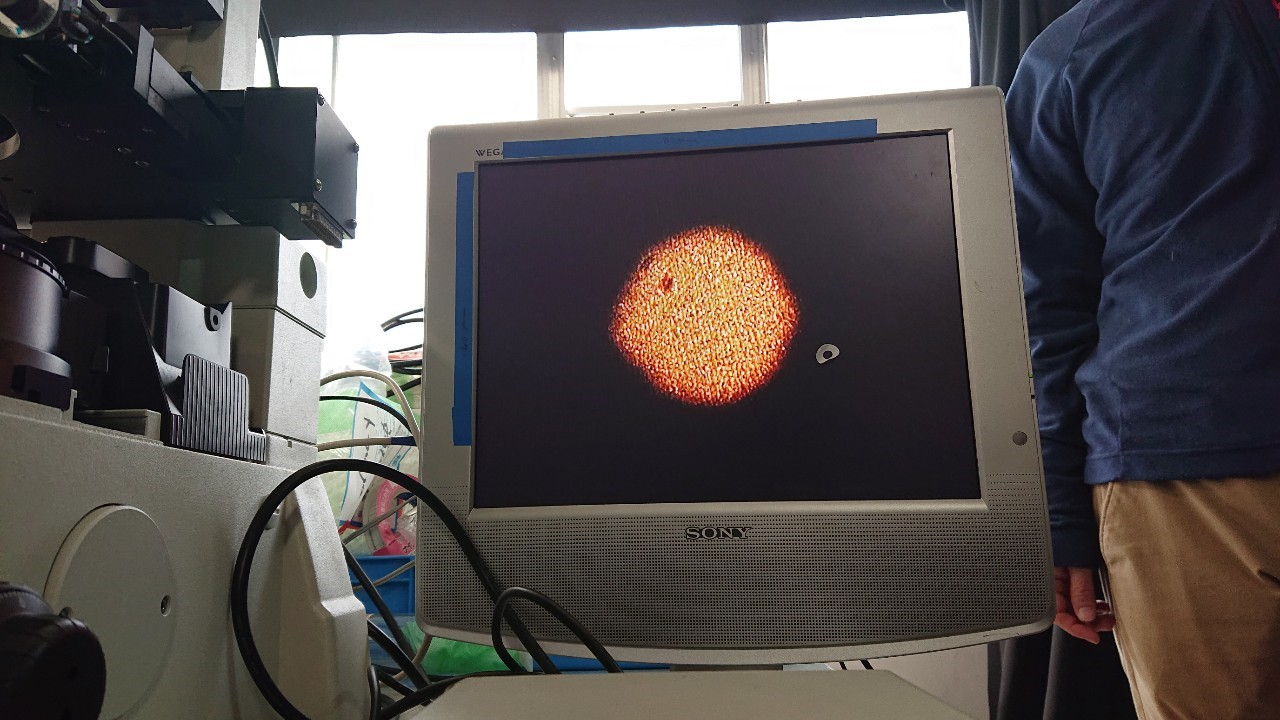
\includegraphics[width=60mm]{fig26.png}
  \end{center}
  \caption{光学顕微鏡で観察した$0.2mm$円形開口}
  \label{fig:26}
 \end{minipage}
 \begin{minipage}{0.45\hsize}
  \begin{center}
   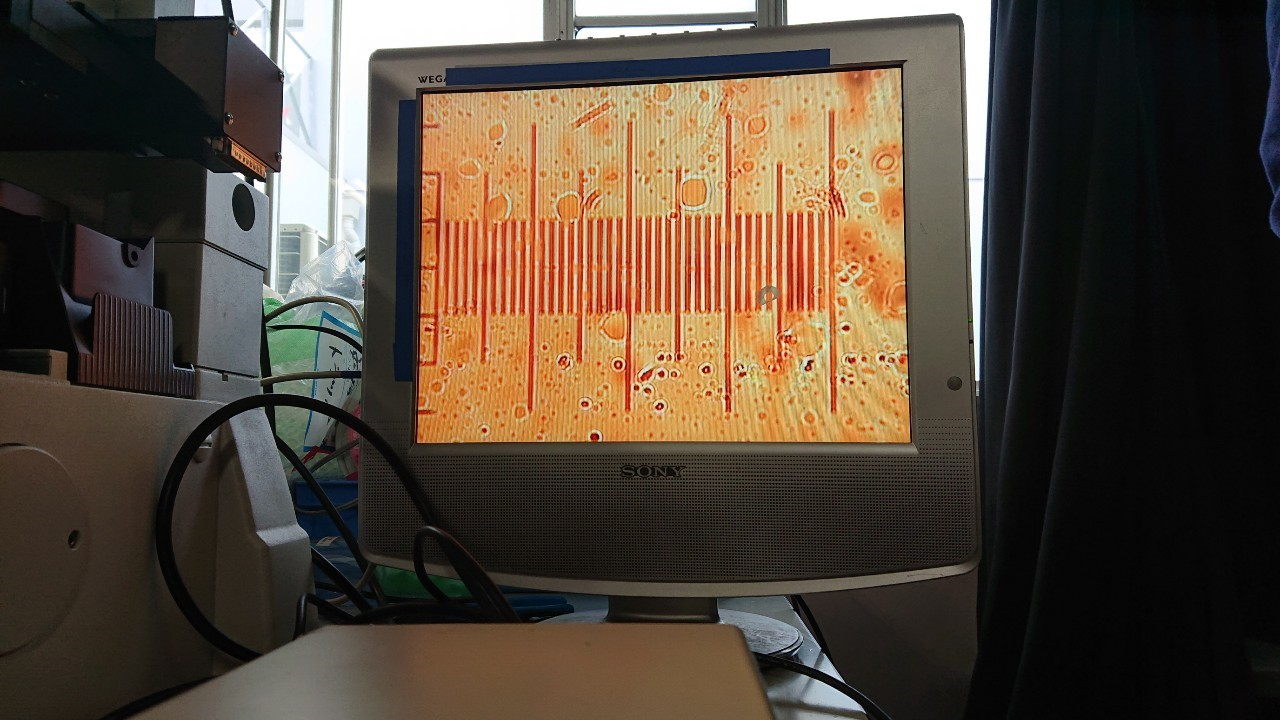
\includegraphics[width=60mm]{fig27.png}
  \end{center}
  \caption{光学顕微鏡で計測した目盛り}
  \label{fig:27}
 \end{minipage}
\end{figure}
\subsubsection{Discussion}
$0.2mm$円形開口の実験値と実測値である0.19mmとの差は比較的小さかった.一方で$0.4mm$円形開口の理論値との差はかなりの開きがあった.
また円形開口のプレートは複数個の開口があったためにそれぞれの円形が偏っていたりしたことも考えられる.
さらに他の要因としてそもそも$D$を算出する際に$sin\theta \simeq tan\theta = r/L$と近似したために実際の値とは異なる結果となった可能性が考えられる.
さらには目測による測定に誤差があったなどの要因も考えられる.
また干渉には開口部の大きさがスクリーンまでの距離に対して十分小さい時に起こるフレネル回折,ビーム源もしくは観測点がビームを回折するものから無限遠に位置する時に起こるフラウンホーファー回折などがあるが今回の実験では観測点はビームを回折する開口に比べて十分大きいと考えられるのでフラウンホーファー回折であると考えられる.
%=============================================================
\subsection{Single Slit}
\subsubsection{Procedure}
基本的には前回と同じ光学系を組み立てる.
今回は円形開口の代わりにシングルスリットをレーザーの前に置く.
以下の図はシングルスリットの光学系である.
今回は$r$,$L$の距離を測定する事によって$\omega$の値を推測する.
またこの実験では$0.1mm$,$0.2mm$二つのスリットを用いてそれぞれ1回ずつ測定を行う.
\begin{figure}[htbp]
 \begin{center}
  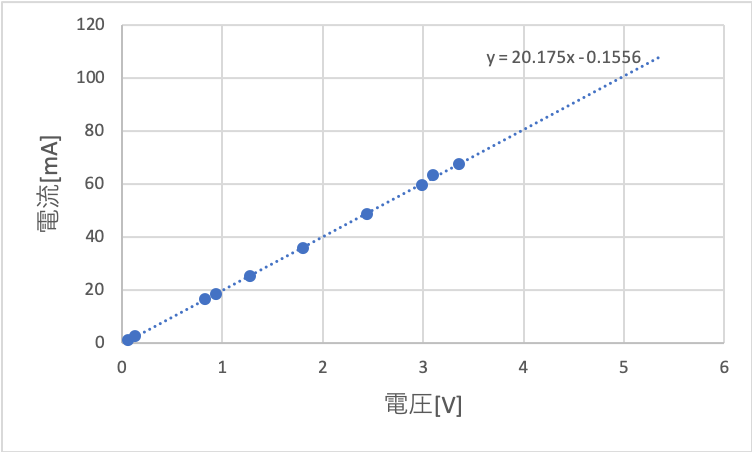
\includegraphics[width=100mm]{fig8.png}
 \end{center}
 \caption{シングルスリットの光学系}
 \label{fig:eight}
\end{figure}\\

またこれらの測定した距離は
\begin{equation}
    sin\theta = \frac{\lambda}{\omega} \label{eq:c}
\end{equation}\\
式(\ref{eq:c})の関係をみたす.
またこの時$\theta$,$D$の値は非常に小さいので$sin\theta \simeq tan\theta = r/L$とみなすことができる.
また今回使用したHe-Ne Laserの波長は$\lambda = 632.8nm$である.
以上より計測値を関係式へ代入してシングルスリットの間隔を推測する.
今回は時間の関係上実際に光学顕微鏡を用いてスリット幅を測定することはできなかった.

\subsubsection{Result}
測定結果から次の表が得られた.
また式(\ref{eq:c})の関係よりスリット幅が大きくなるにつれて干渉縞の間隔は小さくなっていくことが予想される.実際に実験からもこの関係が確かめられた.
\begin{table}[htb]
 \begin{minipage}{0.45\hsize}
  \begin{center}
    \caption{$0.1mm$シングルスリット}
    \begin{tabular}{rrr} \hline
        $r(mm)$ & $L(mm)$ & $\omega(mm)$  \\ \hline
        7.0    & 974 & 0.088\\ \hline
    \end{tabular}
    \label{tab:d}
  \end{center}
 \end{minipage}
 \begin{minipage}{0.45\hsize}
  \begin{center}
    \caption{$0.2mm$シングルスリット}
    \begin{tabular}{rrr} \hline
        $r(mm)$ & $L(mm)$ & $\omega(mm)$  \\ \hline
        3.5    & 974 & 0.176\\ \hline
    \end{tabular}
    \label{tab:e}
  \end{center}
 \end{minipage}
\end{table}

またそれぞれ以下のような干渉模様が観測できた.
\begin{figure}[htbp]
 \begin{minipage}{0.45\hsize}
  \begin{center}
   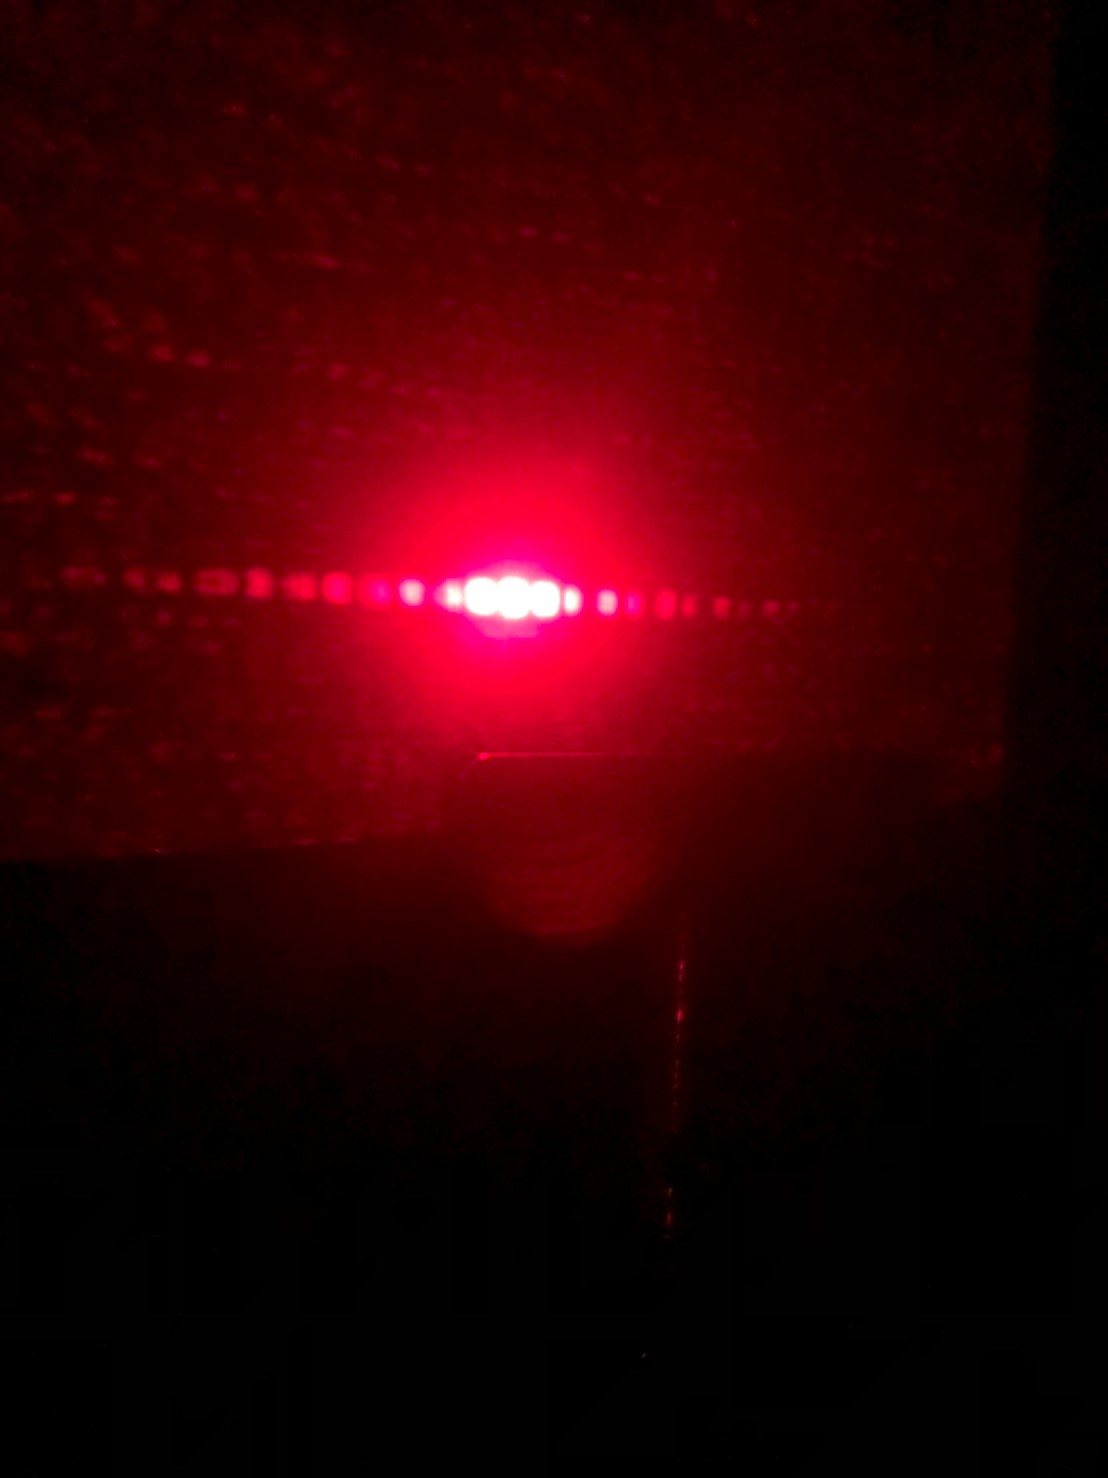
\includegraphics[width=60mm]{fig9.png}
  \end{center}
  \caption{$0.1mm$シングルスリットの干渉縞}
  \label{fig:nine}
 \end{minipage}
 \begin{minipage}{0.45\hsize}
  \begin{center}
   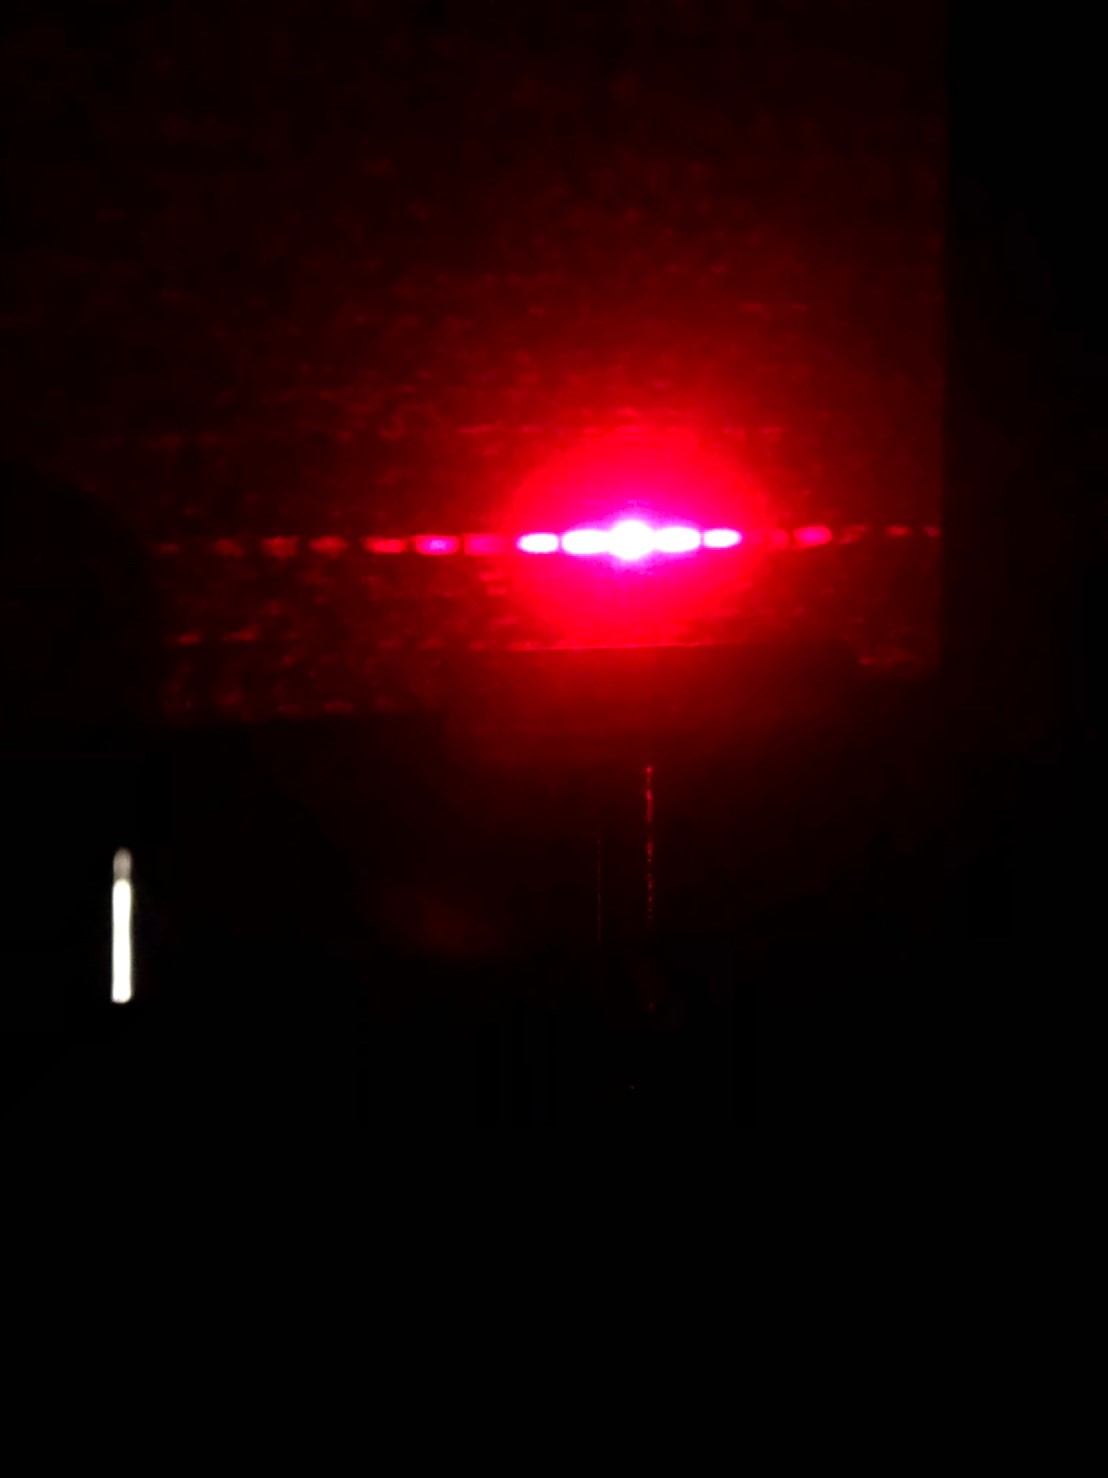
\includegraphics[width=60mm]{fig10.png}
  \end{center}
  \caption{$0.2mm$シングルスリットの干渉縞}
  \label{fig:ten}
 \end{minipage}
\end{figure}
\subsubsection{Discussion}
いずれの結果も理論値よりも$0.02mm$ほど小さくなってしまったのでどちらも目測による計測の時実際の感覚よりも大きく読んでしまった可能性が考えられる.
また光学顕微鏡を用いて実測値を計算していないので実際にスリット幅が0.2mm,0.1mmではなかったために誤差が生じていることも考えられる.
%=============================================================
\subsection{Yong Double Slit}
\subsubsection{Procedure}
光学系を図\ref{fig:eleven}に示すように製作する.
ダブルスリットをビームの経路に置きビーム光を回折させスクリーンに干渉縞を映し観察する.

\begin{figure}[htbp]
 \begin{center}
  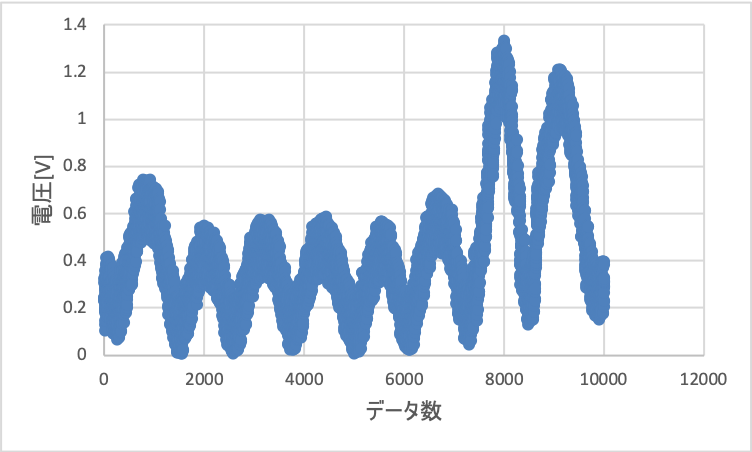
\includegraphics[width=100mm]{fig11.png}
 \end{center}
 \caption{ダブルスリットの光学系}
 \label{fig:eleven}
\end{figure}

またこの時以下の式(\ref{eq:d}),(\ref{eq:f})の関係が成り立つ.それぞれ測定した$\Delta \theta$,$\Delta x$を式に代入することで二つのスリット間隔$d$
を推測する.
また今回は$0.2mm$,$0.1mm$の二つのスリット間隔をを持つダブルスリットに対して一回ずつ計測を行う.
また今回も時間の都合上ダブルスリットの間隔を光学顕微鏡を用いて計りはしなかった.

\begin{equation}
    \Delta\theta = \frac{\Delta x}{R} \label{eq:d}
\end{equation}
\begin{equation}
    \Delta\theta = \frac{\lambda}{d} \label{eq:f}
\end{equation}

\subsubsection{Result}
測定結果から次の表が得られた.

\begin{table}[htb]
 \begin{minipage}{0.45\hsize}
  \begin{center}
    \caption{$0.1mm$ダブルスリット}
    \begin{tabular}{rrr} \hline
        $\Delta x(mm)$ & $R(mm)$ & $d(mm)$  \\ \hline
        7.0    & 974 & 0.088\\ \hline
    \end{tabular}
    \label{tab:f}
  \end{center}
 \end{minipage}
 \begin{minipage}{0.45\hsize}
  \begin{center}
    \caption{$0.2mm$ダブルスリット}
    \begin{tabular}{rrr} \hline
        $\Delta x(mm)$ & $R(mm)$ & $d(mm)$  \\ \hline
        2.8    & 974 & 0.22\\ \hline
    \end{tabular}
    \label{tab:g}
  \end{center}
 \end{minipage}
\end{table}

また以下のような干渉縞が観察された.

\begin{figure}[htbp]
 \begin{minipage}{0.45\hsize}
  \begin{center}
   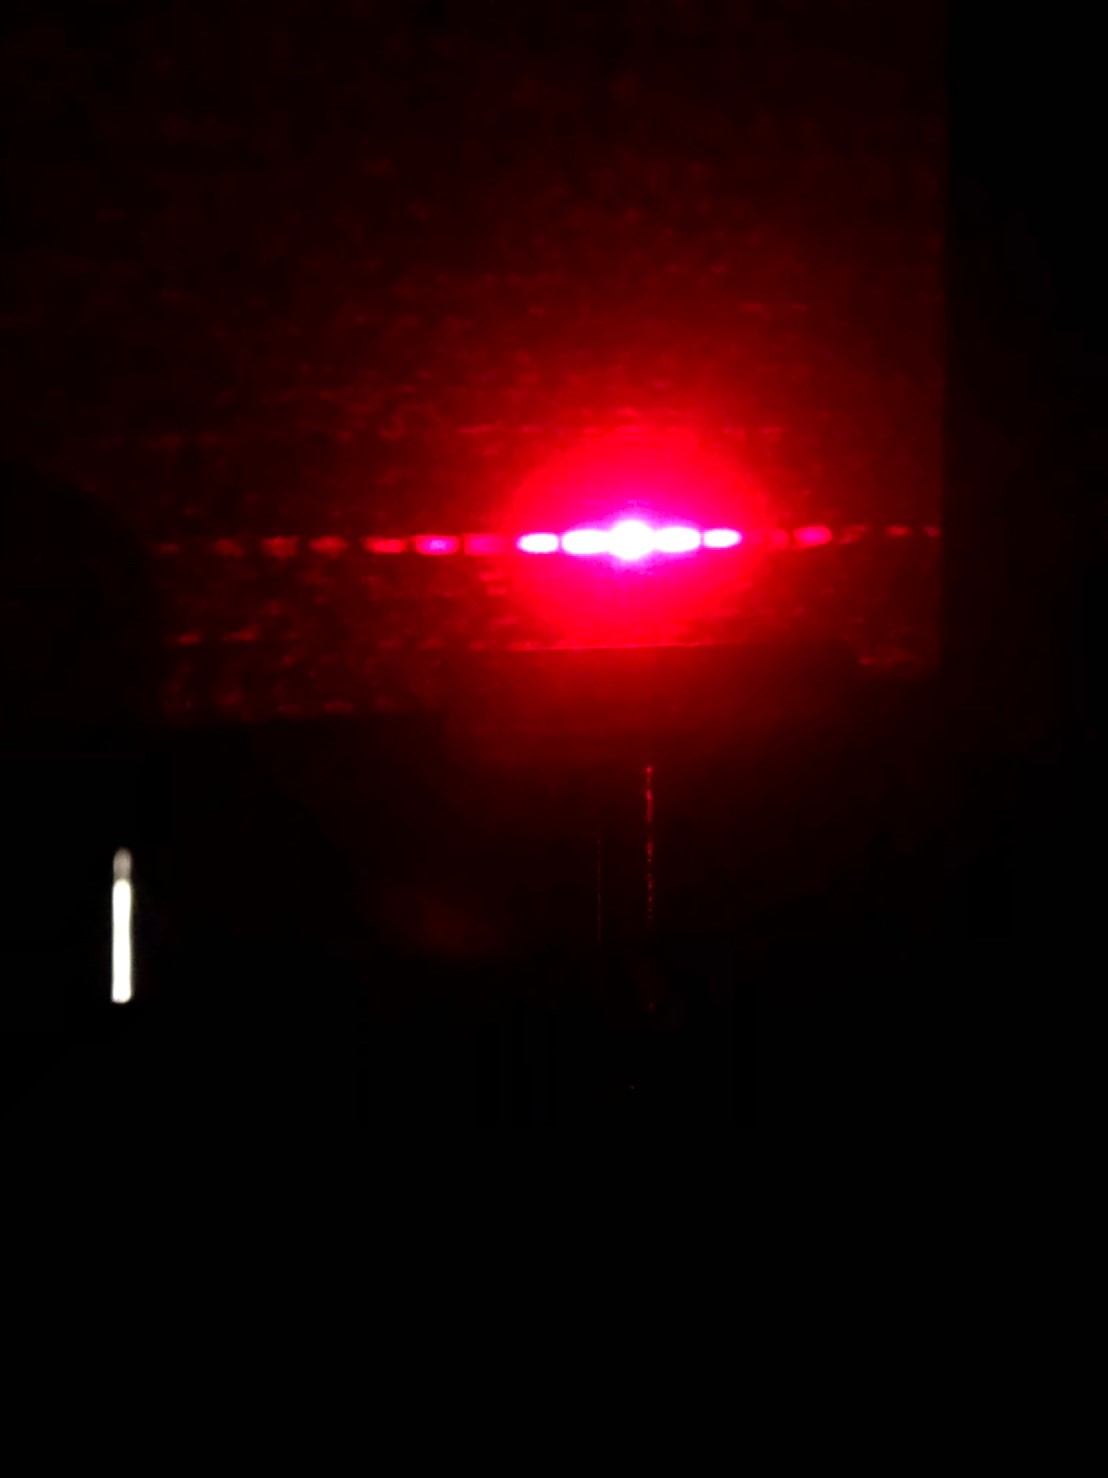
\includegraphics[width=60mm]{fig12.png}
  \end{center}
  \caption{$0.1m$ダブルスリットの干渉縞}
  \label{fig:12}
 \end{minipage}
 \begin{minipage}{0.45\hsize}
  \begin{center}
   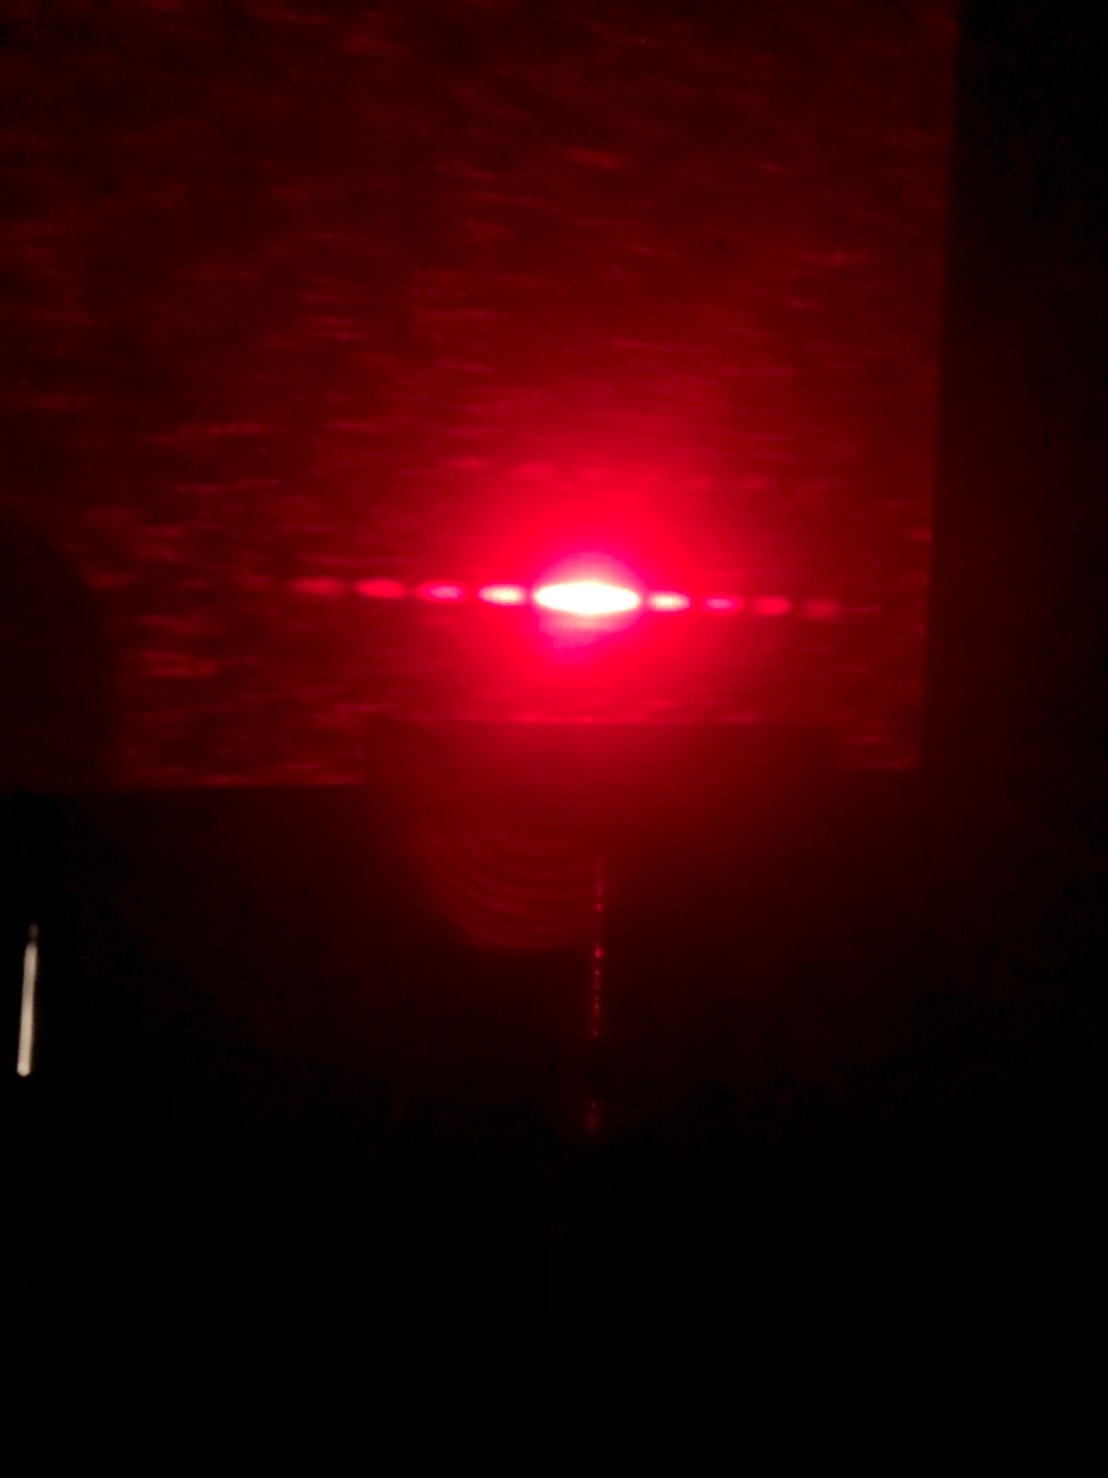
\includegraphics[width=60mm]{fig13.png}
  \end{center}
  \caption{$0.2m$ダブルスリットの干渉縞}
  \label{fig:13}
 \end{minipage}
\end{figure}

\subsubsection{Discussion}
どちらの誤差も$-0.02mm$であったので目測の際に$r$を大きく読んでしまったことなどが考えられる.
またシングルスリットの時と同じような干渉縞が得られたがシングルスリットの方が中心が明るく,ダブルスリットの時は中心から離れた干渉縞でも強度が高かったことが観測された.これはダブルスリットの際は二つのスリットを通過した際にビーム光が素元波となり互いの波が干渉をするためだと考えられる.

%==========================================================
%==========================================================
\newpage
\end{document}
